\lab{Givens rotations and Least squares}{Givens rotations and Least squares}
\objective{Use Givens rotations to find the QR decomposition and use least squares to fit curves to data.}
\label{lab:givens}

In Lab \ref{lab:QRdecomp}, we found the QR decomposition of a matrix using Householder transformations, applying a series of these transformations to a matrix until it was in upper triangular form.
We can use the same strategy to compute the QR decomposition with rotations instead of reflections.

\section*{Givens rotations}

Let us begin with Givens rotations in $\mathbb{R}^2$. 
An arbitrary vector $\x = (a, b)^T$ can be rotated into the span of $e_1$ via an orthogonal transformation. 
In fact, the matrix $T_{\theta} = \begin{pmatrix}\cos \theta & - \sin \theta \\ \sin \theta & \cos \theta \end{pmatrix}$ rotates a vector counterclockwise by $\theta$.
Thus, if $\theta$ is the clockwise-angle between $\x$ and $e_1$, the vector $T_{-\theta}\x$ will be in the span of $e_1$.
We can find $\sin \theta$ and $\cos \theta$ with the formulas $\sin = \frac{\text{opp}}{\text{hyp}}$ and $\cos = \frac{\text{adj}}{\text{hyp}}$, so $\sin \theta = \frac{b}{\sqrt{a^2+b^2}}$ and $\cos \theta =  \frac{a}{\sqrt{a^2+b^2}}$ (see Figure\ref{fig:angle}).
Then 
\[
T_{-\theta}\x = \begin{pmatrix}\cos \theta &  \sin \theta \\ -\sin \theta & \cos \theta \end{pmatrix} \begin{pmatrix} a \\ b \end{pmatrix} = \begin{pmatrix}\frac{a}{\sqrt{a^2+b^2}} & \frac{b}{\sqrt{a^2+b^2}} \\ -\frac{b}{\sqrt{a^2+b^2}} & \frac{a}{\sqrt{a^2+b^2}} \end{pmatrix}\begin{pmatrix} a \\ b \end{pmatrix} = \begin{pmatrix} \sqrt{a^2+b^2} \\ 0 \end{pmatrix}.
\]

\begin{figure}
\begin{center}
\begin{tikzpicture}
\draw[-, thick](-.5,0)--(3,0);
\draw[-, thick](0,-.5)--(0,1.5);
\draw[->, thick, >=stealth'](0,0)--(2.5,1);
\draw[-,thick](2.5,-.2)--(2.5,.2);
\draw[-, thick](-.2,1)--(.2,1);
\node[draw=none](point_b)at(2.5,-.4){$a$};
\node[draw=none](point_a)at(-.4,1){$b$};
\draw[-, thick] (.5,.2)arc [start angle=60, 
	end angle=-20, radius=4.5pt];
\node[draw=none](theta)at(.8, .15){$\theta$};
\end{tikzpicture}
\caption{Rotating clockwise by $\theta$ will send the vector $(a,b)^T$ to the span of $e_1$.}
\label{fig:angle}
\end{center}
\end{figure}



The matrix $T_{\theta}$ above is an example of a $2 \times 2$ Givens rotation matrix. 
In general, the Givens matrix $G(i,j,\theta)$ represents the orthonormal transformation that rotates the 2-dimensional span of $e_i$ and $e_j$ by $\theta$ radians. 
The matrix for this transformation is
\begin{equation*}
G(i,j,\theta) = \begin{pmatrix}
I & 0 & 0 & 0 & 0 \\
0 & c & 0 & -s & 0 \\
0 & 0 & I & 0 & 0 \\
0 & s & 0 & c & 0 \\
0 & 0 & 0 & 0 & I
\end{pmatrix}.
\end{equation*}
This matrix is in block form with $I$ representing the identity matrix, $c=\cos \theta$, and $s=\sin \theta$. 
The $c$'s appear on the $i^{th}$ and $j^{th}$ diagonal entries. 

As before, we can choose $\theta$ so that $G(i,j,\theta)$ rotates a given vector so that its $e_j$-component is 0. 
Such a transformation will only affect the $i^{th}$ and $j^{th}$ entries of any vector it acts on (and thus the $i^{th}$ and $j^{th}$ rows of any matrix it acts on). 



This flexibility makes Givens rotations ideal for some problems.
For example, Givens rotations can be used to solve linear systems defined by sparse matrices by modifying only small parts of the array.
Also, Givens rotations can be used to solve systems of equations in parallel.

The advantages of Givens rotations are that they orthonormal and hence numerically stable (like Householder reflections), and they affect only a small part of the array (like Gaussian elimination).
The disadvantage is that they require a greater number of floating point operations than Householder reflections.
% Accuracy and Stability of Numerical Algorithms, Nicholas J. Higham
In practice, the Givens algorithm is slower than the Householder algorithm, even when it is modified to decrease the number of floating point operations. 
% Fast Plane Rotations With Dynamic Scaling, Anda and Park, SIAM, 1994
However, since Givens rotations can be parallelized, they can be much faster than the Householder algorithm when multiple processors are used.
% Givens and Householder Reductions for Linear Least Squares on a Cluster of Workstations, Omer Egecioglu and Ashok Srinivasan




\subsection*{Givens triangularization}
We can apply Givens rotations to a matrix until it is in upper triangular form, producing a factorization $A = QR$ where $Q$ is a composition of Givens rotations and $R$ is upper triangular.
Similar to the Householder triangularization, when $A$ is square, this decomposition will be the QR decomposition of $A$.

The idea is to iterate through the subdiagonal entries of $A$ in the order depicted by Figure \ref{fig:givens}. 
We zero out the $ij^{th}$ entry with a rotation in the plane spanned by $e_{i-1}$ and $e_i$. 
This rotation is just multiplication by the Givens matrix $G(i-1,i,\theta)$, which can be computed as in the example at the start of the previous section. 
We just set $a=a_{i-1,j}$ and $b=a_{i,j}$, so $c = \cos \theta = a/\sqrt{a^2+b^2}$ and $s = -b/\sqrt{a^2+b^2}$.

\begin{figure}
\begin{center}
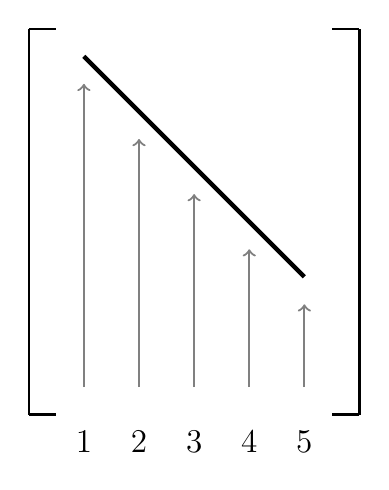
\begin{tikzpicture}[xscale=.7, yscale=.7]
\draw[->, gray, thick](0,0)--(0,5.5);
\draw[->, gray, thick](1,0)--(1,4.5);
\draw[->, gray, thick](2,0)--(2,3.5);
\draw[->, gray, thick](3,0)--(3,2.5);
\draw[->, gray, thick](4,0)--(4,1.5);
\node[draw=none] at(0,-1){\large 1};
\node[draw=none] at(1,-1){\large 2};
\node[draw=none] at(2,-1){\large 3};
\node[draw=none] at(3,-1){\large 4};
\node[draw=none] at(4,-1){\large 5};

\draw[-, ultra thick] (0,6)--(4,2);

\draw[-, thick](-1,-.5)--(-1,6.5);
\draw[-, thick](-1, -.5)--(-.5,-.5);
\draw[-, thick](-1,6.5)--(-.5,6.5);

\draw[-, thick](5,-.5)--(5,6.5);
\draw[-, thick](5,-.5)--(4.5,-.5);
\draw[-, thick](5,6.5)--(4.5,6.5);

%\draw[-, thick](-.5,0)--(3,0);
%\draw[-, thick](0,-.5)--(0,1.5);
%\draw[->, thick, >=stealth'](0,0)--(2.5,1);
%\draw[-,thick](2.5,-.2)--(2.5,.2);
%\draw[-, thick](-.2,1)--(.2,1);
%\node[draw=none](point_b)at(2.5,-.4){$a$};
%\node[draw=none](point_a)at(-.4,1){$b$};
%\draw[-, thick] (.5,.2)arc [start angle=60, 
%	end angle=-20, radius=4.5pt];
%\node[draw=none](theta)at(.8, .15){$\theta$};
\end{tikzpicture}
\caption{This figure illustrates the order in which to zero out subdiagonal entries in the Givens triangularization algorithm. 
The heavy black line is the main diagonal of the matrix. 
Entries should be zeroed out from bottom to top in each column, beginning with the leftmost column.}
\label{fig:givens}
\end{center}
\end{figure}


For example, on a $2 \times 3$ matrix we may perform the following operations:

\def\mc#1{\multicolumn{1}{c|}{#1}}
\def\lc#1{\multicolumn{1}{|c}{#1}}
\[
\begin{array}{ccccccc}
\begin{pmatrix}
*&*\\
*&*\\
*&*
\end{pmatrix}
&
\underrightarrow{G(2,3,\theta_1)}
&\begin{pmatrix}
&*&*&\\ \cline{2-3}
&\lc{*}&\mc{*}&\\
&\lc{0}&\mc{*}& \\ \cline{2-3}
\end{pmatrix}
&
\underrightarrow{G(1,2,\theta_2)}
& \begin{pmatrix} \cline{2-3}
&\lc{*}&\mc{*}&\\
&\lc{0}&\mc{*}&\\ \cline{2-3}
&0&*&
\end{pmatrix}
&
\underrightarrow{G(2,3,\theta_3)}
&\begin{pmatrix}
*&*&\\ \cline{2-2}
\mc{0}&\mc{*}&\\
\mc{0}&\mc{0}&\\ \cline{2-2}
\end{pmatrix}
\end{array}
\]
At each stage, the boxed entries are those modified by the previous transformation. 
The final transformation $G(2,3,\theta_3)$ operates on the bottom two rows, but since the first two entries are zero, they are unaffected. 
Assuming that at the $ij^{th}$ stage of the algorithm, $a_{ij}$ is nonzero, Algorithm \ref{Alg:givens} computes the Givens triangularization of a matrix..


\begin{algorithm}
\begin{algorithmic}[1]
\caption{Givens Triangularization. Return an orthogonal matrix $Q$ and an upper triangular matrix $R$ satisfying $A = QR$.}
\label{Alg:givens}
\Procedure{Givens Triangularization}{$A$}
\State $R \gets \text{copy}(A)$
\State $Q \gets I_A$
\State $G \gets \text{empty}((2,2))$
\For{$0\leq j < n$}
    \For{$ m \geq i > j$}
      \State $a, b \gets R_{i-1,j}, R_{i,j}$
      \State $G \gets [[a, b],[-b,a]]/\sqrt{a^2+b^2}$
      \State $R_{i-1:i+1, j:} = GR_{i-1:i+1, j:}$
      \State $Q_{i-1:i+1,:} = GQ_{i-1:i+1,:}$
    \EndFor
\EndFor
\State \pseudoli{return} $Q^T, R$
\EndProcedure
\end{algorithmic}
\end{algorithm}

Notice that in Algorithm \ref{Alg:givens}, we \emph{do not} actually create the matrices $G(i,j,\theta)$ and multiply them by the original matrix.
Instead we modify only those entries of the matrix that are affected by the transformation. As an additional way to save memory, it is possible to modify this algorithm so that $Q$ and $R$ are stored in the original matrix $A$.
\begin{comment}
An interesting side-note is that each Givens rotation can be represented as a single floating point number, so, when operating in place, $Q$ can be stored entirely in the lower triangular portion of the array on which we are operating by storing each rotation in the entry that it zeroes out.
A similar approach would to store Householder reflectors in the columns they zero out.
In either case, we can represent the QR decomposition of an array using only the memory that was originally used to store the array itself.
This is similar to the approach  for computing the LU decomposition entirely in place.
These representations of $Q$ and $R$ can be used in various ways to perform matrix multiplication by $Q$, $Q^T$ and $R$ as needed.
\end{comment}







\begin{comment}
\begin{itemize}[$\bullet$]

\item Make $R$ a copy of $A$ and $Q$ an identity array of the appropriate size.

\item Make an empty $2 \times 2$ array $G$ that will be used to apply the Givens rotations.

\item For each column:

  \begin{itemize}[$\bullet$]

  \item For each row below the main diagonal (starting at the bottom of the column):

    \begin{itemize}[$\bullet$]

    \item If the leading entry of this row is not zero (i.e. if its absolute value is within a given tolerance):

      \begin{itemize}[$\bullet$]

      \item Compute $c$ and $s$ using the entry in the current row and column and the entry immediately above it.

      \item Use $c$ and $s$ to construct the matrix $G$.

      \item Get a slice of $R$ of the current row and the row above it that includes the columns from the current column onward.
      Multiply it in place by $G$ to zero out the leading nonzero entry of the current row.

      \item Get a slice of $Q$ of the current row and the row above it and apply $G$ to it as well. (Strictly speaking, you do not need to operate over these entire rows, but the slicing needed to avoid the extra computation is a little more involved, so we will not include that here.)

      \end{itemize}

    \end{itemize}

  \end{itemize}

\item Return $Q^T$ and $R$.

\end{itemize}
\end{comment}


\begin{problem}
\label{prob:Givens}
Write a function that computes the Givens triangularization of a matrix, using Algorithm \ref{Alg:givens}. 
Assume that at the $ij^{th}$ stage of the algorithm, $a_{ij}$ will be nonzero.
\end{problem}


\begin{problem}
\label{prob:givens_hessenberg}
Modify your solution to Problem \ref{prob:Givens} to compute the Givens triangularization of an upper Hessenberg matrix, making the following changes:
\begin{enumerate}
\item Iterate through the first subdiagonal from left to right. (These are the only entries that need to be zeroed out.)
\item Line 10 of Algorithm \ref{Alg:givens} updates $Q$ with the current Givens rotation $G$. Decrease the number of entries of $Q$ that are modified in this line. Do this by replacing $Q_{i-1:i+1, :}$ with $Q_{i-1:i+1, :k_i}$ where $k_i$ is some appropriately chosen number (dependent on $i$) such that $Q_{i-1:i+1, k_i:}=0$.
\end{enumerate}
Hint: Here is how to generate a random upper Hessenberg matrix on which to test your function.
The idea is to generate a random matrix and then zero out all entries below the first subdiagonal.
\begin{lstlisting}
import numpy as np
import scipy.linalg as la
from math import sqrt
A = np.random.rand(500, 500)

# We do not need to modify the first row of A
# la.triu(A[1:]) zeros out all entries below the diagonal of A[1:]
A[1:] = la.triu(A[1:])

# A is now upper Hessenberg
\end{lstlisting}

\begin{comment}
What is the computational order of  complexity for this problem?
Approximately for what $m$ is your implementation as fast as the general QR decomposition built in to \li{scipy.linalg} for computing the QR decomposition of an upper Hessenberg matrix?
\end{comment}
\end{problem}

\begin{comment}
\begin{problem}
\label{prob:givens_hessenberg_modified}
You may have noticed that matrix multiplication by $Q$ is generally a $\mathcal{O} \left( n^3 \right)$ algorithm, while the application of these individual Givens rotations is a $\mathcal{O} \left( n^2 \right)$ algorithm.
Write a modified version of your solution to Problem \ref{prob:givens_hessenberg} called \li{givens2_mod} which returns 
an $(n-1) \times 2 \times 2$ array containing the computed values for $G$ at each step in the algorithm in the order in which they are applied to the upper Hessenberg array $H$.

Write two more functions \li{apply_Q} and \li{apply_QT} which, using the matrix of Givens rotations, perform left multiplication 
by $Q$ and $Q^{-1}$, respectively, on some other input array $B$.
Left multiplication by $Q^{-1}$ can be done by applying each of the Givens rotations to $B$ the same way you did to $H$ to compute its QR factorization.
Left multiplication by $Q$ can be done by applying the transpose of the Givens rotations to their corresponding portions of $B$, but in the reverse order.
Notice that you will have to apply each Givens rotation across the full width of the rows it operates on since you do not know anything about the content of $B$.

For around what size of matrices is direct multiplication by $Q$ slower than this method of multiplying by $Q$?
For timing purposes, make a random upper Hessenberg matrix, compute its QR decomposition using the function you just wrote and your solution to Problem \ref{prob:givens_hessenberg}, then time how long it takes to left multiply a random square array by $Q$ using the function you just wrote and the \li{dot} method of NumPy arrays.

Note: the functions you just wrote can be used to perform right multiplication as well since $B Q = \left(Q^T B^T \right)^T$ and $B Q^T = \left( Q B^T \right)^T$.
\end{problem}
\end{comment}



\section*{Least Squares}

A linear system $A\x=\b$ is \emph{overdetermined} if it has no solutions. 
In this situation, the \emph{least squares solution} is a vector $\widehat{\x}$ hat is ``closest'' to a solution. 
By definition, $\widehat{\x}$ is the vector such that $A\widehat{\x}$ will equal the projection of $\b$ onto the range of $A$. 
We can compute $\widehat{\x}$ by solving the \emph{Normal Equation} $A^HA\widehat{\x} = A^H\b$ (see [TODO: ref textbook] for a derivation of the Normal Equation).

%TODO: update this section, esp the homework problem, once we know how QR is being taught
\subsection*{Solving the normal equation}
If $A$ is full rank, we can use its QR decomposition to solve the normal equation. 
In many applications, $A$ is usually full rank, including when least squares is used to fit curves to data.

It can be shown that if $A=QR$ is the QR decomposition of $A$, then $\widehat{\x}$ solves the normal equation if and only if $R\widehat{\x} = Q^T \b$ ([TODO: ref hw problem in textbook]). 
Since $R$ is upper triangular, we can solve this equation quickly with back substitution. 

%TODO: This problem might need a hint. It is harder to code than it looks.
\begin{problem}
Write a function that accepts a matrix $A$ and a vector $b$ and returns the least squares solution to $Ax=b$.
Use the QR decomposition as outlined above.
Your function should use SciPy's functions for QR decomposition and for solving triangular systems, which are \li{la.qr()} and \li{la.solve_triangular()}, respectively.
\end{problem}

\subsection*{Using least squares to fit curves to data}
The least squares solution can be used to find the curve of a chosen type that best fits a set of points. 

\subsubsection*{Example 1: Fitting a line}
For example, suppose we wish to fit a general line $y=mx+b$ to the data set $\{(x_k, y_k)\}_{k=1}^n$. 
When we plug the constants $(x_k, y_k)$ into the equation $y=mx+b$, we get a system of linear equations in the unknowns $m$ and $b$. 
This system corresponds to the matrix equation
\[
\begin{pmatrix}
x_1 & 1\\
x_2 & 1\\
x_3 & 1\\
\vdots & \vdots\\
x_n & 1
\end{pmatrix}
\begin{pmatrix}
m\\
b
\end{pmatrix}=
\begin{pmatrix}
y_1\\
y_2\\
y_3\\
\vdots\\
y_n
\end{pmatrix}.
\]
Because this system has two unknowns, it is guaranteed a solution if it has two or fewer equations. 
In applications, there will usually be more than two data points, and these will probably not lie in a straight line, due to measurement error. 
Then the system will be overdetermined. 
The least squares solution to this equation will be a slope $\widehat{m}$ and $y$-intercept $\widehat{b}$ that produce a line $y = \widehat{m}x+\widehat{b}$ which best fits our data points.



%DO: spring constant as an example of this
% circle fit
% mention in this situation A will usually be full rank.
%todo: least squares and invertibiility.







Let us do an example with some actual data. Imagine we place different loads on a spring and measure the displacement, recording our results in the table below.
%TODO: get data points that are not so close to an actual line
\begin{table}
\begin{tabular}{c|c|c|c|c|c|c|c}
displacement (cm)& 1.04  &2.03  &2.95  &3.92  &5.06  &6.00  &7.07  \\ \hline
load (dyne) & 3.11&  6.01&  9.07&  11.99 &  15.02&  17.91&  21.12\\
\end{tabular}
\end{table}

Hooke's law from physics says that the displacement $x$ should be proportional to the load $F$, or $F = kx$ for some constant $k$.
The equation $F=kx$ describes a line with slope $k$ and $F$-intercept 0.
So the setup is similar to the setup for the general line we discussed above, except we already know $b=0$
When we plug our seven data points $(x,F)$ pairs into the equation $F=kx$, we get seven linear equations in $k$, corresponding to the matrix equation
\[
\begin{pmatrix}
1.04\\
2.03\\
2.95\\
3.92\\
5.06\\
6.00\\
7.07\\
\end{pmatrix}
\begin{pmatrix}k\end{pmatrix} =
\begin{pmatrix}
3.11 \\
6.01\\
9.07\\
11.99\\
15.02\\
17.91\\
21.12\\
\end{pmatrix}.
\]
We expect such a linear system to be overdetermined, and in fact it is: the equation is $1.04k = 3.11$ which implies $k=2.99$, but the second equation is $2.03k = 6.01$ which implies $k=2.96$.

We can't solve this system, but its least squares solution is a ``best'' choice for $k$.
We can find the least squares solution with the SciPy function \li{linalg.lstlsq()}. 
This function returns a tuple of several values, the first of which is the least squares solution.
\begin{lstlisting}
>>> A = np.vstack([1.04,2.03,2.95,3.92,5.06,6.00,7.07])
>>> b = np.vstack([3.11,6.01,9.07,11.99,15.02,17.91,21.12])
>>> k = la.lstsq(A, b)[0]
>>> k
array([[ 2.99568294]])
\end{lstlisting}
Hence, to two decimal places, $k = 3.00$.
We plot the data against the best-fit line with the following code, whose output is in Figure \ref{fig:spring_fit}


\begin{lstlisting}
>>> from matplotlib import pyplot as plt
>>> x0 = np.linspace(0,8,100)
>>> y0 = k[0]*x0
>>> plt.plot(A,b,'*',x0,y0)
>>> plt.show()
\end{lstlisting}

\begin{figure}
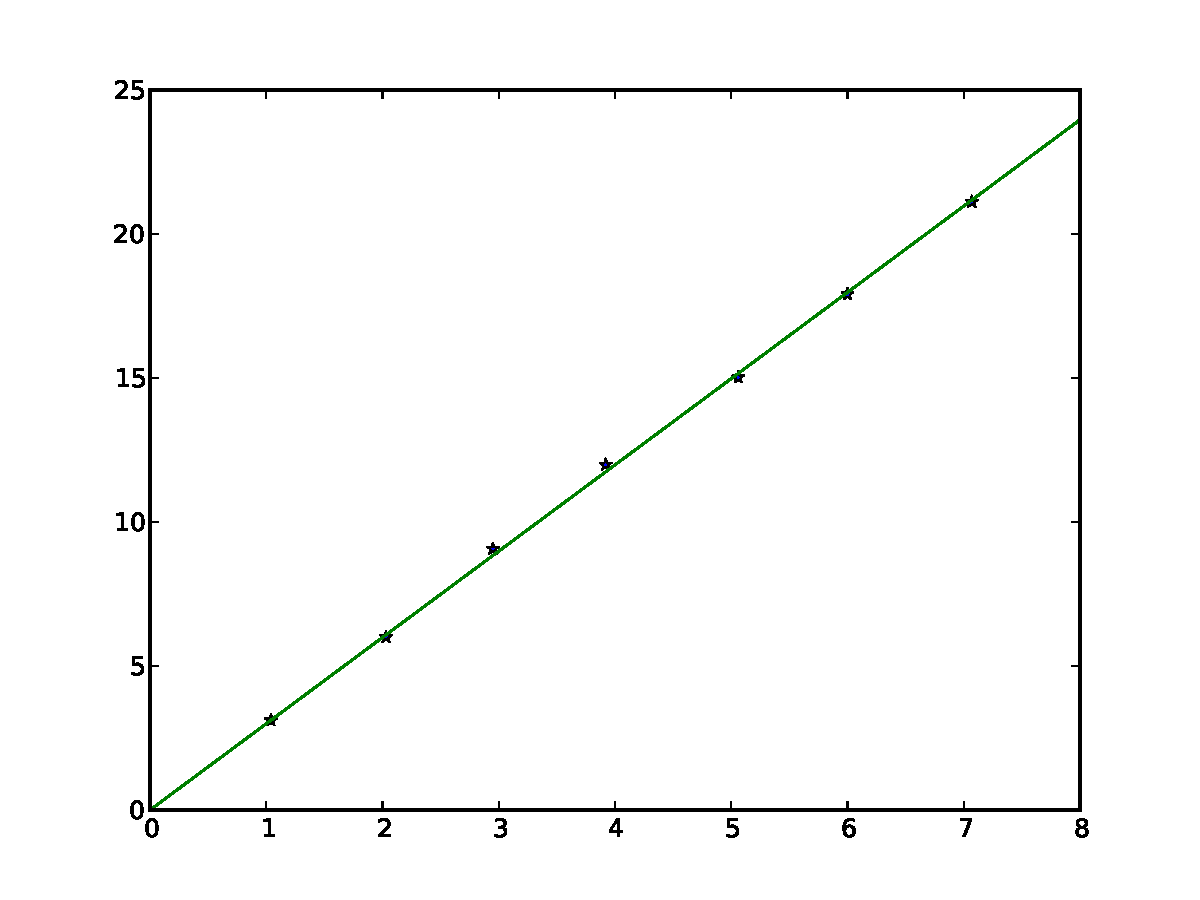
\includegraphics[width=\textwidth]{line_lstsq}
\caption{The graph of the spring data together with its linear fit.}
\label{fig:spring_fit}
\end{figure}

%TODO: find more interesting data and make a sample plot
\begin{problem}
Load the \li{linepts} array from the file \texttt{data.npz}. The following code stores this array as \li{linepts}.
\begin{lstlisting}
linepts = np.load('data.npz')['linepts']
\end{lstlisting}
The \li{linepts} array has two columns corresponding to the $x$ and $y$ coordinates of some data points.
\begin{enumerate}
\item Use least squares to fit the line $y=mx+b$ to the data.
\item Plot the data and your line on the same graph.
\end{enumerate}
\end{problem}






%
%\section*{General Line Fitting}
%
%Suppose that we wish to fit a general line, that is $y=m x+b$, to the data set
%$\{(x_k,y_k)\}^n_{k=1}$.  Assume that the line does not cross through the origin,
%as in the previous example.  Then we seek both a slope and a $y$-intercept.
%In this case, we set up the following linear system $A x = b$, or more precisely
%\[
%\begin{pmatrix}
%x_1 & 1\\
%x_2 & 1\\
%x_3 & 1\\
%\vdots & \vdots\\
%x_n & 1
%\end{pmatrix}
%\begin{pmatrix}
%m\\
%b
%\end{pmatrix}=
%\begin{pmatrix}
%y_1\\
%y_2\\
%y_3\\
%\vdots\\
%y_n
%\end{pmatrix}.
%\]
%Note that $A$ has rank $2$ as long as not all of the $x_k$ values are the same.
%Hence, the least squares solution
%is given by
%$$
%\widehat{x} = (A^HA)^{-1}A^Hb.
%$$
%In what sense does this solution give us the best fit line for the data? Recall that since $A$ is injective,
%the matrix $A(A^HA)^{-1}A^H$ is an orthogonal projector onto the range of $A$, which means that
%$A(A^HA)^{-1}A^Hb = A\widehat{x}$ is the closest vector (with respect to the 2-norm) to $b$ that lies in the
%range of $A$. That is, $\widehat{x}$ minimizes the error between $Ax$ and $b$, where the error is given
%by the distance between these vectors, $\|b-Ax\|_2$. Another way to say this is that $\widehat{x}$ gives the
%values $m$ and $b$ for which the sum of the squares of the distances from each data point $y_k$ to the value
%$y = mx_k + b$ is as small as possible.


\subsubsection*{Example 2: Fitting a circle}
Now suppose we wish to fit a general circle to a data set $\{(x_k, y_k)\}_{k=1}^n$. Recall that the equation of a circle with radius $r$ and center $(c_1,c_2)$ is
\begin{equation}
\label{circle}
(x-c_1)^2 + (y-c_2)^2 = r^2.
\end{equation}
What happens when we plug a data point into this equation? Suppose $(x_k, y_k)=(1,2)$.
\footnote{You don't have to plug in a point for this derivation, but it helps us remember which symbols are constants and which are variables.} Then
\begin{equation*}\label{equ:example}
5 = 2c_1+4c_2+(r^2-c_1^2-c_2^2).
\end{equation*}
To find $c_1$, $c_2$, and $r$ with least squares, we need \emph{linear} equations. 
Then Equation \ref{equ:example} above is not linear because of the $r^2$, $c_1^2$, and $c_2^2$ terms. 
We can do a trick to make this equation linear: create a new variable $c_3$ defined by $c_3 = r^2-c_1^2-c_2^2$. 
Then Equation \ref{equ:example} becomes
\[
5=2c_1+4c_2+c_3,
\]
which \emph{is} linear in $c_1$, $c_2$, and $c_3$. Since $r^2 = c_3+c_1^2+c_2^2$, after solving for the new variable $c_3$ we can also find $r$.

For a general data point $(x_k, y_k)$, we get the linear equation
\[
2c_1x_k+2c_2y_k+c_3=x_k^2+y_k^2.
\]
Thus, we can find the best-fit circle from the least squares solution to the matrix equation

\begin{equation}\label{equ:circle_fit}
\begin{pmatrix}
2 x_1 & 2 y_1 & 1\\
2 x_2 & 2 y_2 & 1\\
\vdots & \vdots & \vdots \\
2 x_n & 2 y_n & 1
\end{pmatrix}
\begin{pmatrix}
c_1\\
c_2\\
c_3
\end{pmatrix}=
\begin{pmatrix}
x_1^2 + y_1^2\\
x_2^2 + y_2^2\\
\vdots\\
x_n^2 + y_n^2
\end{pmatrix}.
\end{equation}
If the least squares solution is $\widehat{c_1}, \widehat{c_2}$, $\widehat{c_3}$, then the best-fit circle is
\[
(x-\widehat{c_1})^2 + (y-\widehat{c_2})^2 = \widehat{c_3}+\widehat{c_1}^2+\widehat{c_2}^2.
\]


Let us use least squares to find the circle that best fits the following nine points:
%TODO: get data points that are not so close to an actual circle
\begin{table}
\begin{tabular}{c||c|c|c|c|c|c|c|c|c}
$x$& 134  &104 &34  &-36  &-66  &-36  &34 &104 &  134  \\ \hline
$y$& 76&  146&  176&  146 &  76&  5& -24 & 5 & 76\\
\end{tabular}
\end{table}


We enter them into Python as a $9\times 2$ array.
\begin{lstlisting}
>>> P = np.array([[134,76],[104,146],[34,176],[-36,146],
                  [-66,76],[-36,5],[34,-24],[104,5],[134,76]])
\end{lstlisting}

We compute $A$ and $b$ according to Equation \ref{equ:circle_fit}.
\begin{lstlisting}
>>> A = np.hstack((2*P, np.ones((9,1))))
>>> b = (P**2).sum(axis=1)
\end{lstlisting}

Then we use SciPy to find the least squares solution.
\begin{lstlisting}
>>> c1, c2, c3 = la.lstsq(A, b)[0]
\end{lstlisting}

We can solve for $r$ using the relation $r^2 = c_3+c_1^2+c_2^2$.
\begin{lstlisting}
>>> r = sqrt(c1**2 + c2**2 + c3)
\end{lstlisting}

A good way to plot a circle is to use polar coordinates. 
Using the same variables as before, the equation for a general circle is $x=r\cos(\theta)+c_1$ and $y=r\sin(\theta)+c_2$. 
With the following code we plot the data points and our best-fit circle using polar coordinates. 
The resulting image is Figure \ref{fig:circle}.
\begin{lstlisting}
# In the polar equations for a circle, theta goes from 0 to 2*pi.
>>> theta = np.linspace(0,2*np.pi,200)
>>> plt.plot(r*np.cos(theta)+c1,r*np.sin(theta)+c2,'-',P[:,0],P[:,1],'*')
>>> plt.show()
\end{lstlisting}

\begin{figure}
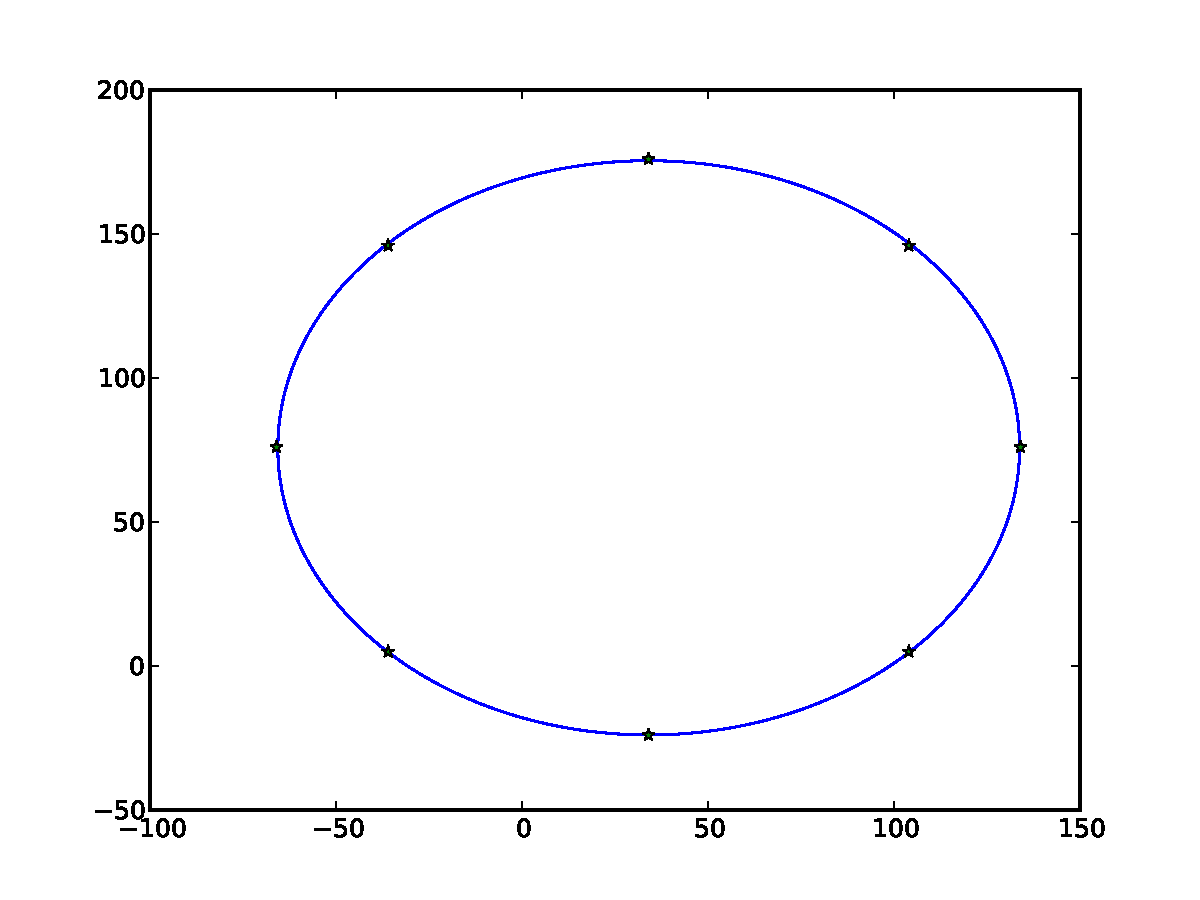
\includegraphics[width=\textwidth]{circle.pdf}
\caption{The graph of the some data and its best-fit circle.}
\label{fig:circle}
\end{figure}

\begin{comment}
\begin{problem}
Write a function \li{fitCircle} that does the following.
Load the \texttt{circlepts} array from \texttt{data.npz}.
This consists of two columns corresponding to the $x$ and $y$ values of a given
data set.  Use least squares to find the center and radius of the circle that best
fits the data.  Then plot the data points and the circle on the same graph.
The function should return nothing.
\end{problem}
\end{comment}

%TODO: figure out how to plot this problem
\begin{problem}
\leavevmode
\begin{enumerate}
\item Load the \texttt{ellipsepts} array from \texttt{data.npz}. This array has two columns corresponding to the $x$ and $y$ coordinates of some data points.
\item Use least squares to fit an ellipse to the data. 
The general equation for an ellipse is
\[
ax^2 + bx + cxy + dy + ey^2 = 1.
\]
You should get  $0.087$, $-0.141$,  $0.159$, $-0.316$, $0.366$ for $a, b, c, d,$ and $e$ respectively.
%\item Plot the data and your line on the same graph.
\end{enumerate}
\end{problem}

%TODO: keep this?
\begin{comment}
In these Least Squares problems, we have found best fit lines and ellipses relative to the 2-norm.
It is possible to generalize the idea of best fit curves relative to other norms.
See Figure \ref{Fig:ellipse} for an illustration of this.

\begin{figure}[h]
\label{ellipsefit}
\centering
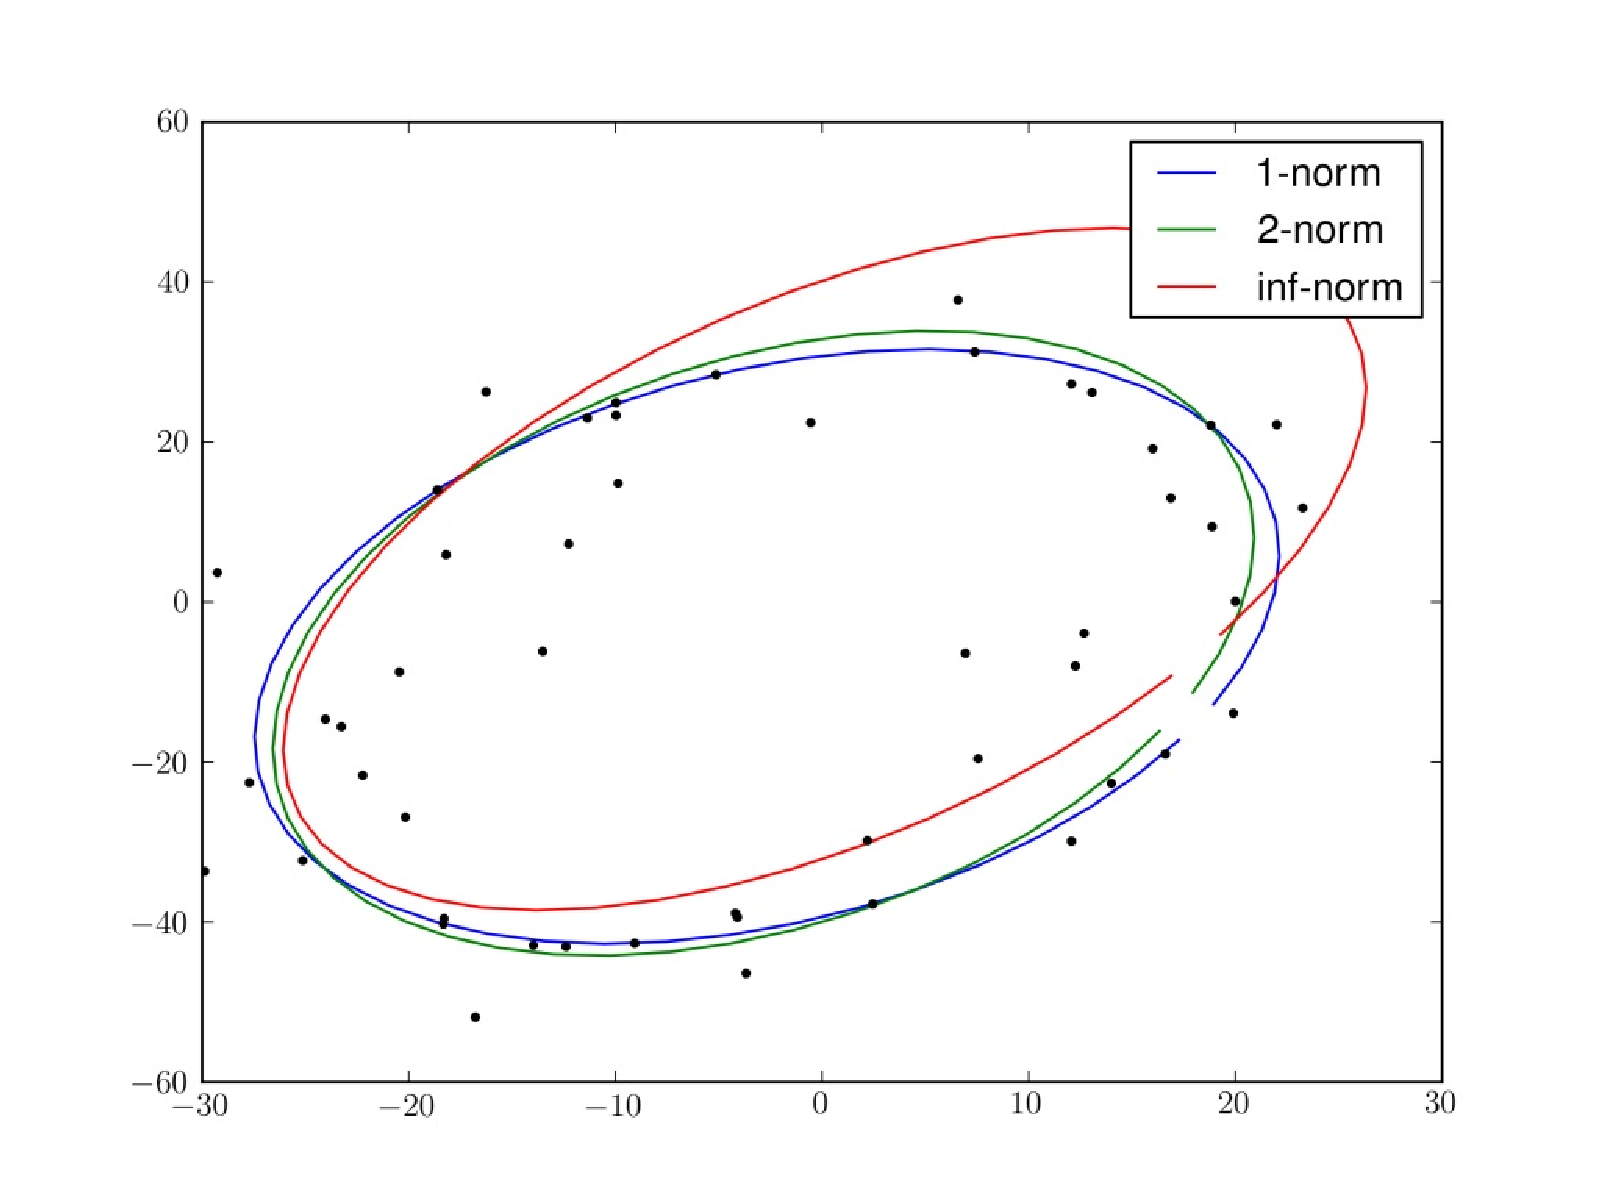
\includegraphics[width=\textwidth]{ellipsefit.pdf}
\caption{Fitting an ellipse using different norms.}
\label{Fig:ellipse}
\end{figure} 
\end{comment}

\begin{comment}
\section*{Loading Data from .npz Files}
For Least Squares problems as well as in many other contexts, loading data is often a necessary step before
proceeding with further analysis. Here we briefly review another data format in Python and the commands used
to load the data.

A \li{.npz} file is a compressed binary file that contains an archive of NumPy data structures.
A given file may therefore contain several arrays, each array associated with a unique string that identifies it.
When you load a \li{.npz} file in Python, a dictionary-like object is returned, and you can access the data by
providing the appropriate key. Note that when you load a \li{.npz} file, you must also be sure to close it when
you are finished. This is taken care of automatically if you use the \li{with ... as} keywords.

As an example, suppose that we have a file named \li{grades.npz} that contains several arrays, each giving the
homework scores of a particular student in a particular class. Assuming that one of the arrays is associated with
the key \li{'Abe'}, we can load this array in the following way:

\begin{lstlisting}
>>> with np.load('grades.npz') as grades:
>>>     abe_grades = grades['Abe']
>>> abe_grades
array([ 10.,  10.,  10.,  10.,  10.,  10.,  10.,  10.,  10.,  10.])
\end{lstlisting}

You will need to apply this technique in the next problem.

\end{comment}
